\justifying 

\begin{problem}{1}
	Вантаж масою $m_1 = 10$ кг зрівноважено двома іншими вантажами $m_2$ та $m_3$, причому $m_2 = 18$ кг. Нитка, яка втримує вантаж $m_3$, напрямлена від точки А горизонтально. Визначити масу вантажу $m_3$ та кут $\alpha$. (див. рис. \ref{fig:gon353})
	\begin{figure}[h!]
		\centering
		\begin{subfigure}{.4\textwidth}
			\centering
			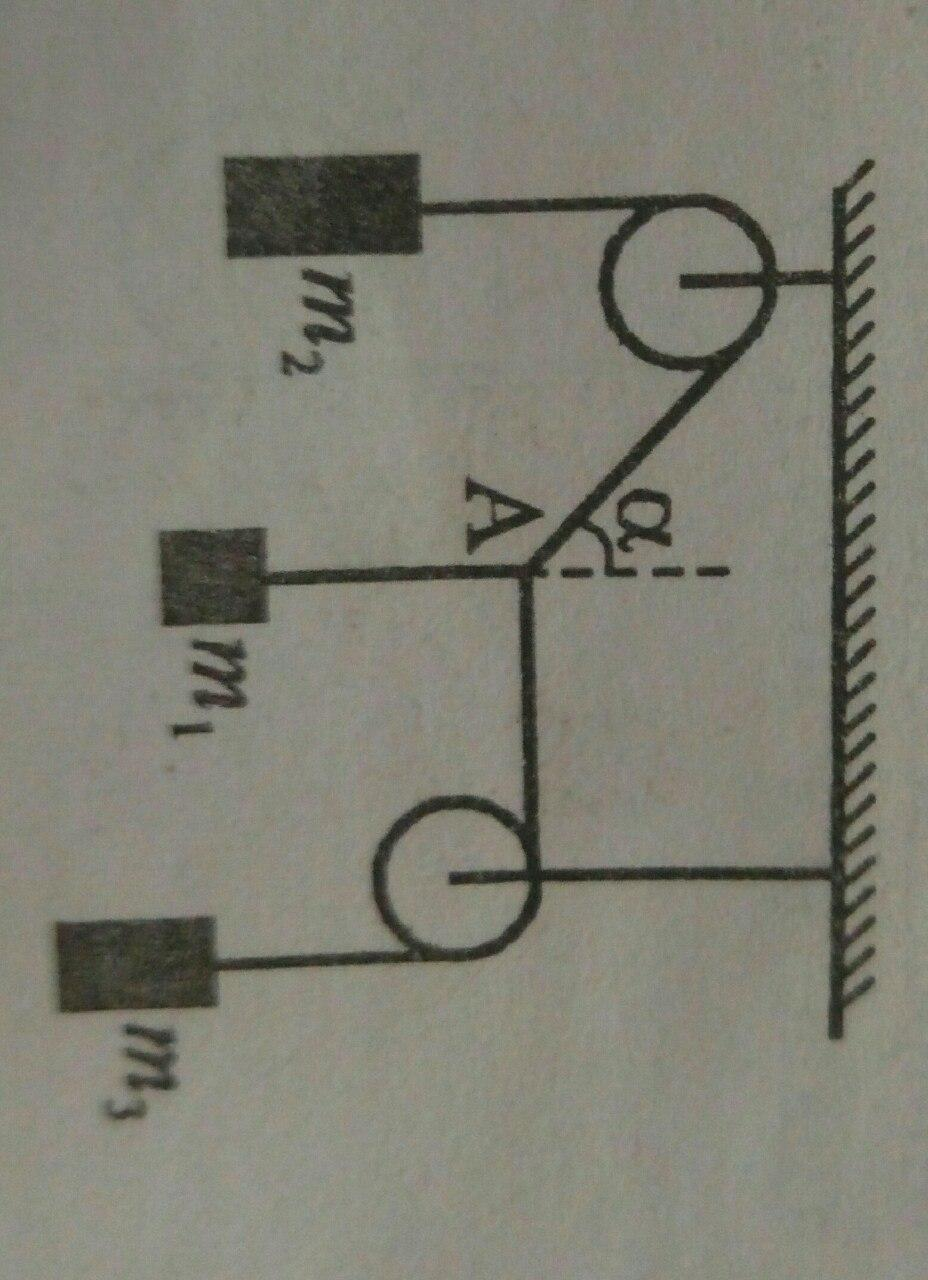
\includegraphics[width=0.5\linewidth]{class7/gon_353}
			\caption{}
			\label{fig:gon353}
		\end{subfigure}
		\begin{subfigure}{.4\textwidth}
			\centering
			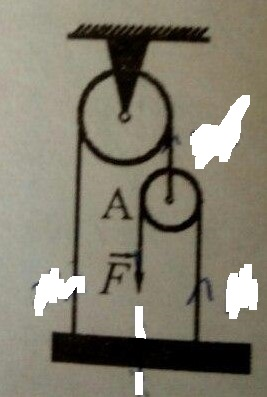
\includegraphics[width=0.5\linewidth]{class7/gon_269}
			\caption{}
			\label{fig:gon269}
		\end{subfigure}
		\begin{subfigure}{.4\textwidth}
			\centering
			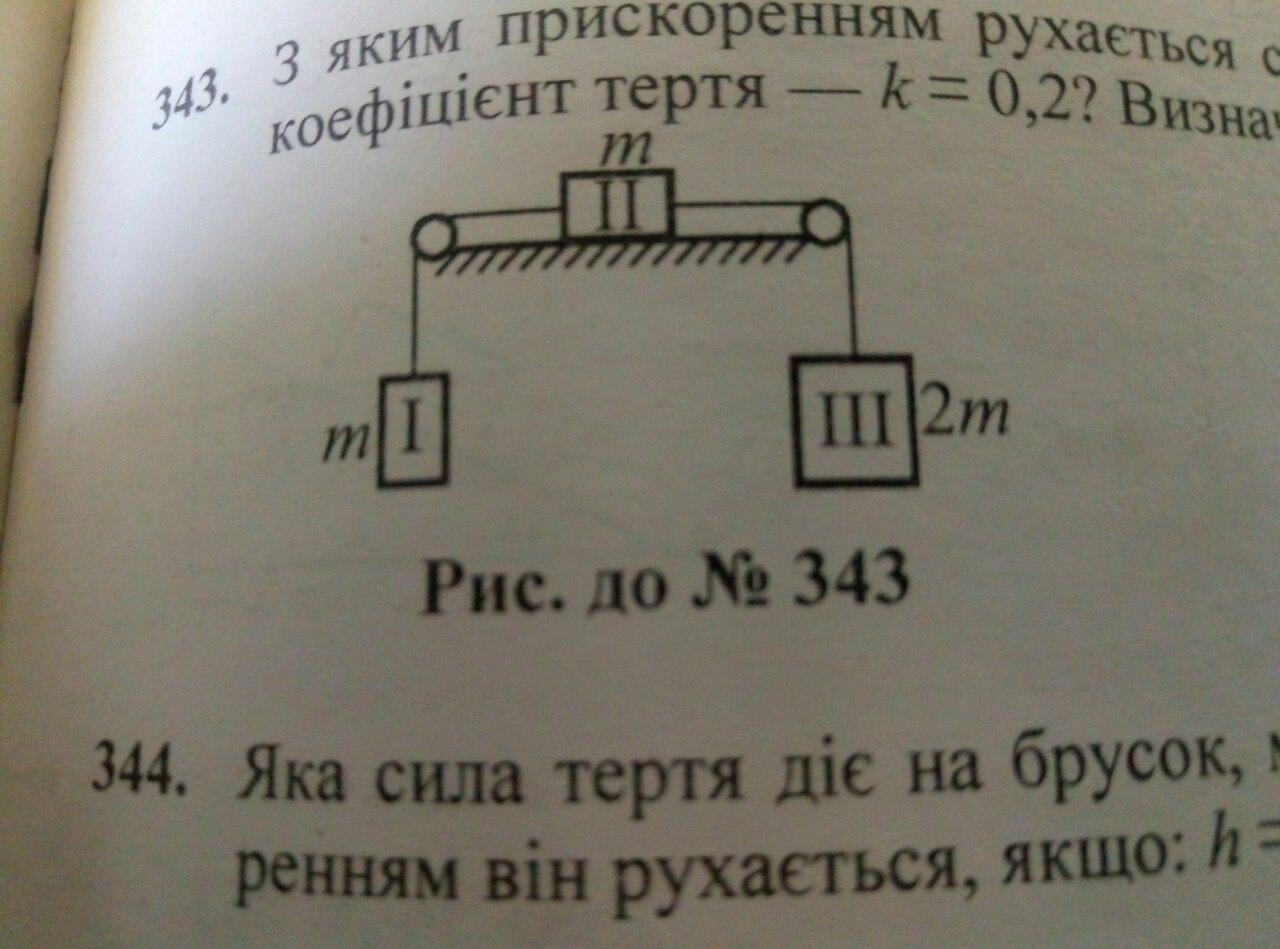
\includegraphics[width=0.5\linewidth]{class7/gon_343}
			\caption{}
			\label{fig:gon343}
		\end{subfigure}
		\begin{subfigure}{.4\textwidth}
			\centering
			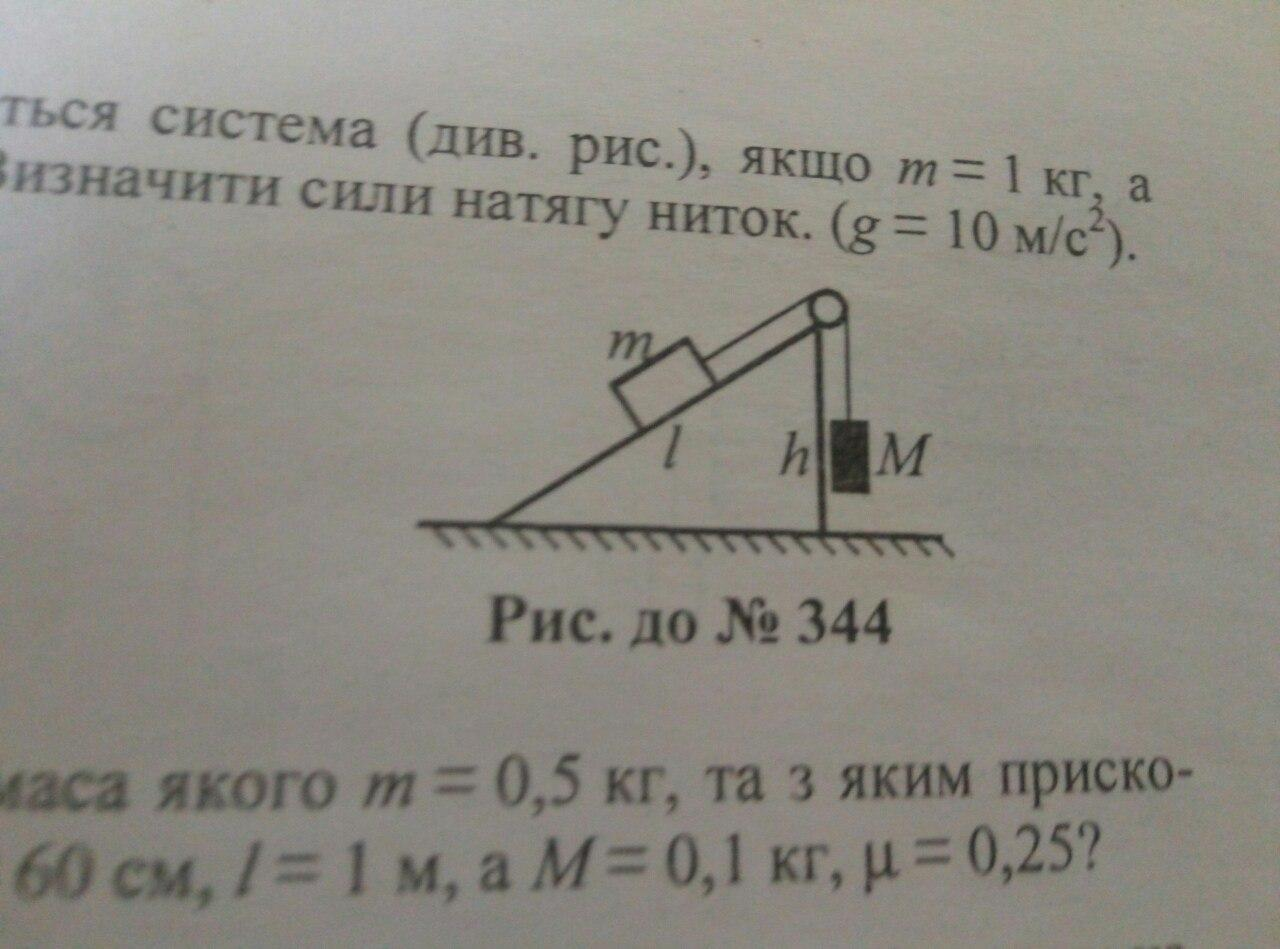
\includegraphics[width=0.5\linewidth]{class7/gon_344}
			\caption{}
			\label{fig:gon344}
		\end{subfigure}
		\begin{subfigure}{.4\textwidth}
			\centering
			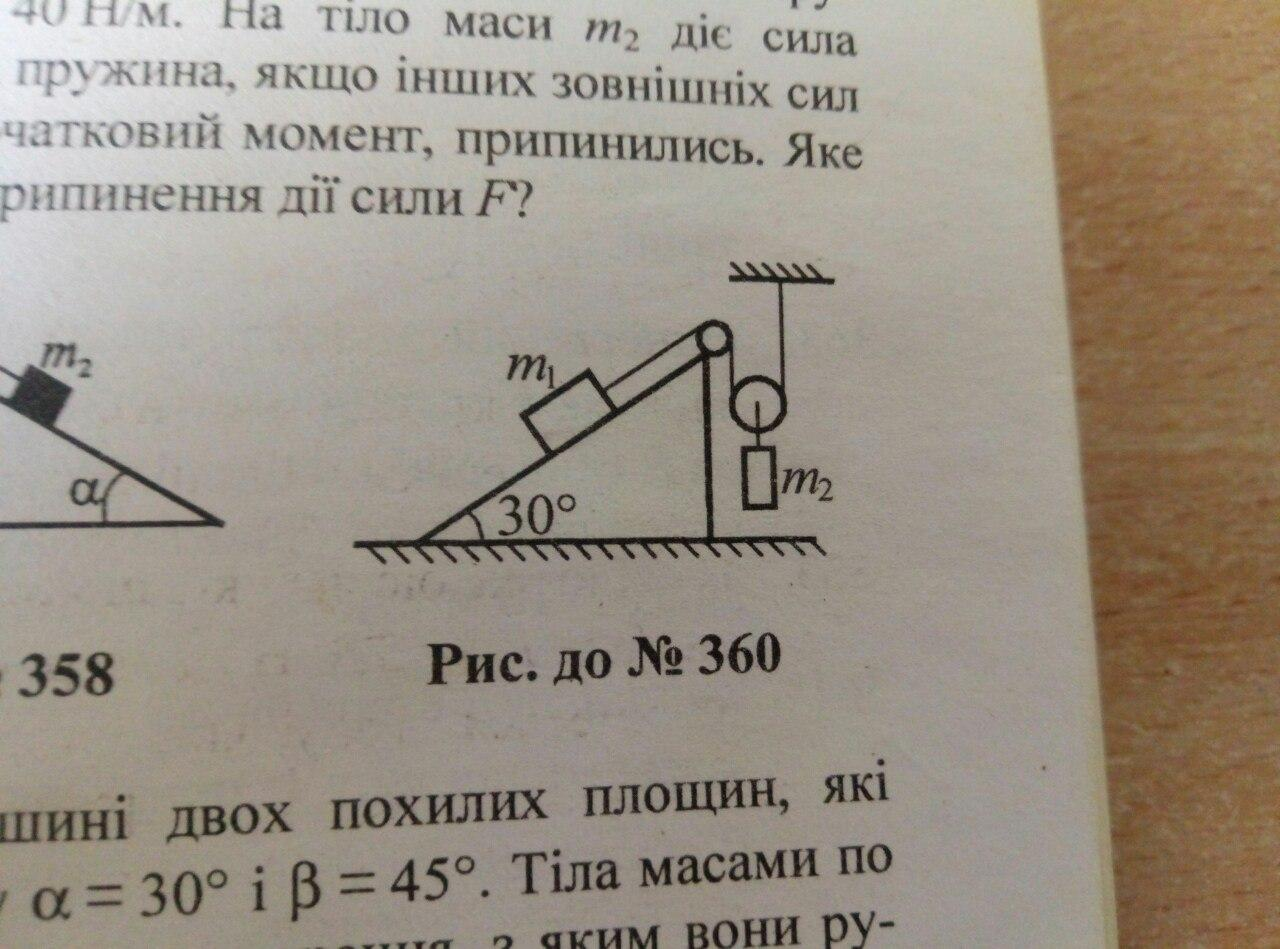
\includegraphics[width=0.5\linewidth]{class7/gon_360}
			\caption{}
			\label{fig:gon360}
		\end{subfigure}
		\begin{subfigure}{.4\textwidth}
			\centering
			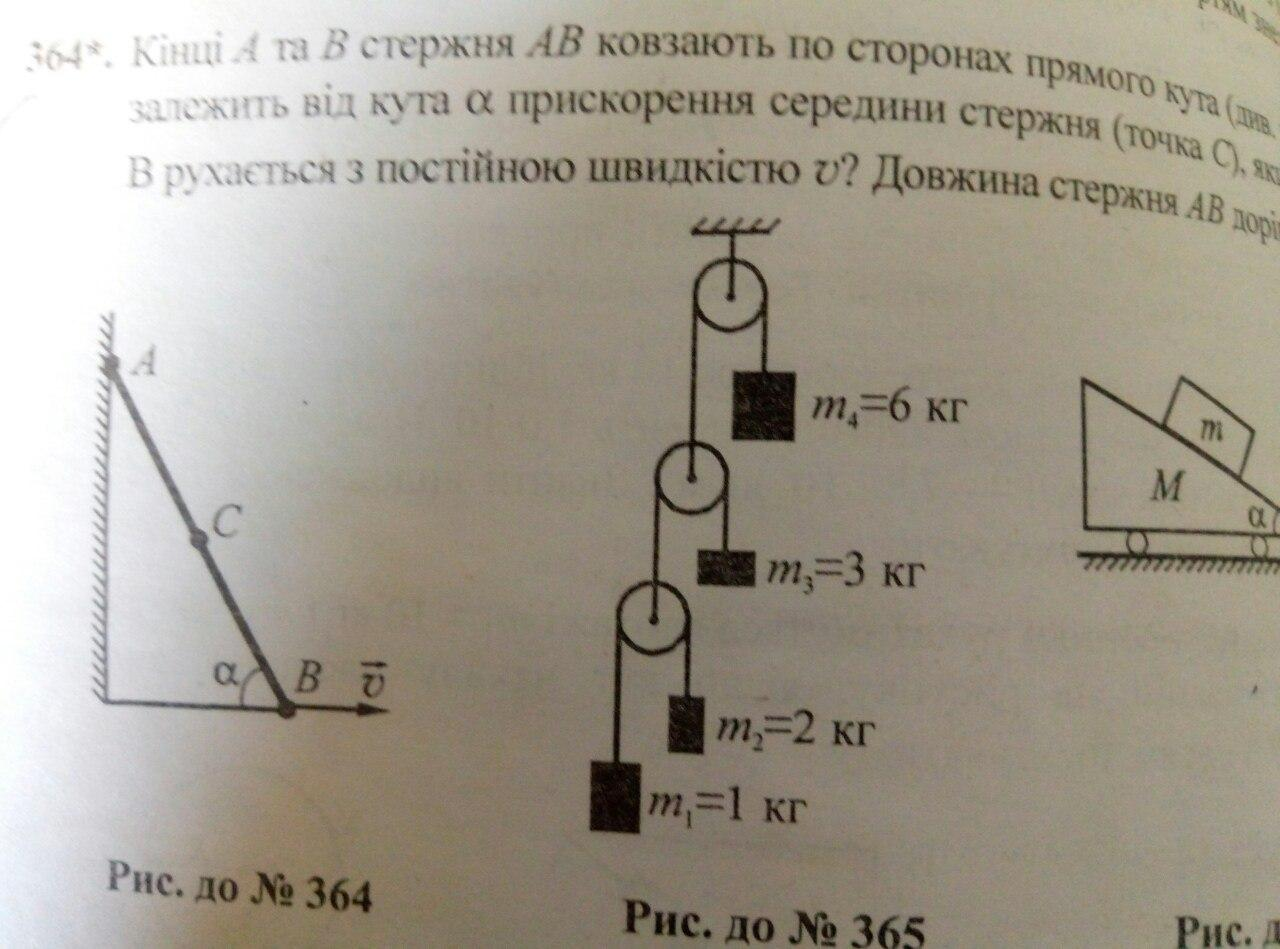
\includegraphics[width=0.5\linewidth]{class7/gon_365}
			\caption{}
			\label{fig:gon365}
		\end{subfigure}
		\begin{subfigure}{.4\textwidth}
			\centering
			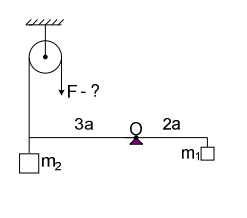
\includegraphics[width=0.5\linewidth]{class7/lev_379}
			\caption{}
			\label{fig:lev379}
		\end{subfigure}
	\caption{}
	\end{figure}
	
\end{problem}



\begin{problem}{3}
	
	\begin{figure}[h!]
	\centering
	\begin{subfigure}{.4\textwidth}
		\centering
		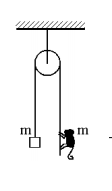
\includegraphics[width=0.5\linewidth]{class7/lev_445}
		\caption{}
		\label{fig:lev445}	
	\end{subfigure}
	\begin{subfigure}{.4\textwidth}
		\centering
		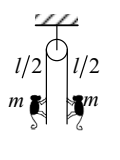
\includegraphics[width=0.5\linewidth]{class7/lev_447}
		\caption{}
		\label{fig:lev447}
	\end{subfigure}
	\begin{subfigure}{.4\textwidth}
		\centering
		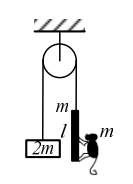
\includegraphics[width=0.5\linewidth]{class7/lev_449}
		\caption{}
		\label{fig:lev449}
	\end{subfigure}
	\begin{subfigure}{.4\textwidth}
		\centering
		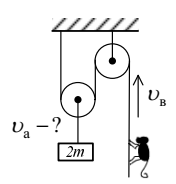
\includegraphics[width=0.5\linewidth]{class7/lev_451}
		\caption{}
		\label{fig:lev451}
	\end{subfigure}
	\begin{subfigure}{.4\textwidth}
		\centering
		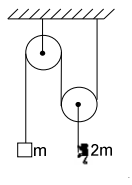
\includegraphics[width=0.5\linewidth]{class7/lev_453}
		\caption{}
		\label{fig:lev453}
	\end{subfigure}
	\begin{subfigure}{.4\textwidth}
		\centering
		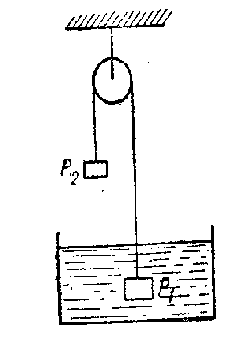
\includegraphics[width=0.5\linewidth]{class7/gonch_150}
		\caption{}
		\label{fig:gonch150}
	\end{subfigure}
	\caption{}
\end{figure}
\end{problem}

\begin{problem}{4}
	Яка сила тертя діє на брусок, маса якого $m = 0.5$ кг, та з яким прискоренням він рухається. якщо: $h = 60$ см, $l = 1$ м, а $M = 0.1$ кг, $\mu = 0.25$ (див. рис. \ref{fig:gon344})
\end{problem}

\begin{problem}{5}
	З яким прискоренням рухатимуться вантажі $m_1 = 10$ кг та $m_2 = 5$ кг у системі, показаній на рисунку, якщо кут нахилу площини дорівнює $\alpha = 30^{\circ}$? (див. рис. \ref{fig:gon360})
\end{problem}





\begin{problem}{8}
	Через легкий блок без тертя перекинута легка мотузка, на якій зрівноважені мавпа та тіло однакової маси. Мавпа починає рухатись вгору зі швидкістю $2~\dfrac{\text{м}}{\text{c}}$ \underline{відносно мотузки}. Через скільки часу мавпа досягне блока? Довжина мотузки $16$ м. Як зміниться відповідь, якщт швидкість руху мавпи буде $2~\dfrac{\text{м}}{\text{c}}$ \underline{відносно Землі} (див. рис. \ref{fig:lev445})	

\end{problem}



\begin{problem}{10}
	Через легкий блок без тертя перекинута легка мотузка, на одному кінці якої висить тіло масою $2m$, а до другого кінця прикріплено жердину довжиною $l$, масою $m$, в нижній точці якої сидить
	мавпа масою $m$. Система перебуває у рівновазі. Мавпа піднімається з нижньої точки жердини у верхню. На яку висоту підніметься
	вантаж масою $2m$? (див. рис. \ref{fig:lev449})
\end{problem}




\begin{problem}{12}
	 У зрівноваженій системі (блоки і мотузки невагомі, тертя немає) тіло $m$ і мавпа $2m$ нерухомі. Мавпа починає рухатись вгору зі швидкістю $6~\dfrac{\text{м}}{\text{c}} $ відносно мотузки. Яка швидкість тіла
	$m$ і як вона напрямлена? (див. рис. \ref{fig:lev453})
\end{problem}



\textbf{Задачі для самостійного розв'язання}

\begin{problem}{2}
	За допомогою системи блоків необхідно підняти колоду масою $m$. З якою силою $F$ потрібно тягнути за кінець канату А, щоб підняти колоду? (див. рис. \ref{fig:gon269})
\end{problem}


\begin{problem}{3}
	З яким прискоренням рухається система. якшо $m = 1$ кг, а коефіцієнт тертя -- $k = 0.2$? Визначити силу натягу ниток (див. рис. \ref{fig:gon343})
\end{problem}

\begin{problem}{6}
	Визначити прискорення вантажу у системі, зображеній на рисунку. Масою блоків та ниток знехтувати. (див. рис. \ref{fig:gon365})	
\end{problem}

\begin{problem}{7}
	З якою силою треба тягнути мотузку, щоб система буда у рівновазі? $m_1 = 1$ кг, $m_2 = 5$ кг (див. рис. \ref{fig:lev379})
\end{problem}

\begin{problem}{9}
	Через легкий блок без тертя перекинута легка мотузка, на якій зрівноважені дві мавпи однакової маси (спочатку система знаходилась у спокої). Мавпи починають рухатись вгору: перша зі швидкістю $v$ відносно мотузки, а лруга зі швидкістю $2v$ відносно мотузки. За який час мавпи досягнуть блока? (див. рис. \ref{fig:lev447})
\end{problem}

\begin{problem}{11}
	У системі тіл, зображених на малюнку, мотузки і блоки невагомі, тертя немає. Тіло $2m$ і мавпа $m$ нерухомі.
	Мавпа починає повзти вгору по мотузці. Швидкість мавпи відносно мотузки $6~\dfrac{\text{м}}{\text{c}} $. Яка швидкість тіла відносно Землі? (див. рис. \ref{fig:lev451})
\end{problem}

\begin{problem}{13}
	Блок з важками $P_1 = 9.8$ H i $P = 5.88$ H підвішено над широкою посудиною. Нехтуючи опором рідини, визначити її густину, якщо відомо, що система рухається з прискоренням $0.2~\dfrac{\text{м}}{\text{c}^2} $ і густина речовини першого важка дорівнює $2700 ~\dfrac{\text{кг}}{\text{м}^3}$. (див. рис. \ref{fig:gonch150})
	
	(Вказівка: на тіло, занурене у воду діє сила Архімеда, яка напрямлена до поверхні рідини і рівна $F_A = \rho_p gV$, $\rho_p $ - густина рідини, $V$ - об'єм зануреної частини тіла)	
\end{problem}